\documentclass[12pt]{article}
\usepackage[paperwidth=15.8in,paperheight=6.8in,margin=0.18in]{geometry}
\usepackage[T1]{fontenc}
\usepackage{lmodern}
\usepackage{amsmath}
\usepackage{xcolor}
\usepackage{tikz}
\usetikzlibrary{arrows.meta,positioning,shapes.geometric}

\definecolor{psidblue}{HTML}{1E3A5F}
\definecolor{psidline}{HTML}{D1D5DB}
\definecolor{psidpanel}{HTML}{F7FAFC}
\definecolor{psidaccent}{HTML}{E8F1FB}
\definecolor{psidgold}{HTML}{A16207}

\pagestyle{empty}
\setlength{\parindent}{0pt}
\setlength{\parskip}{0pt}

\tikzset{
  flowstep/.style={
    rectangle,
    rounded corners=6pt,
    draw=psidblue,
    fill=psidpanel,
    very thick,
    align=center,
    text width=3.6cm,
    minimum height=1cm,
    font=\sffamily\small
  },
  flowwide/.style={flowstep, text width=4.4cm},
  flowresult/.style={flowstep, draw=psidgold!85!black, fill=psidaccent},
  flowarrow/.style={-{Stealth[length=3mm]}, very thick, draw=psidblue}
}

\begin{document}
\thispagestyle{empty}
\centering
\resizebox{0.98\textwidth}{!}{%
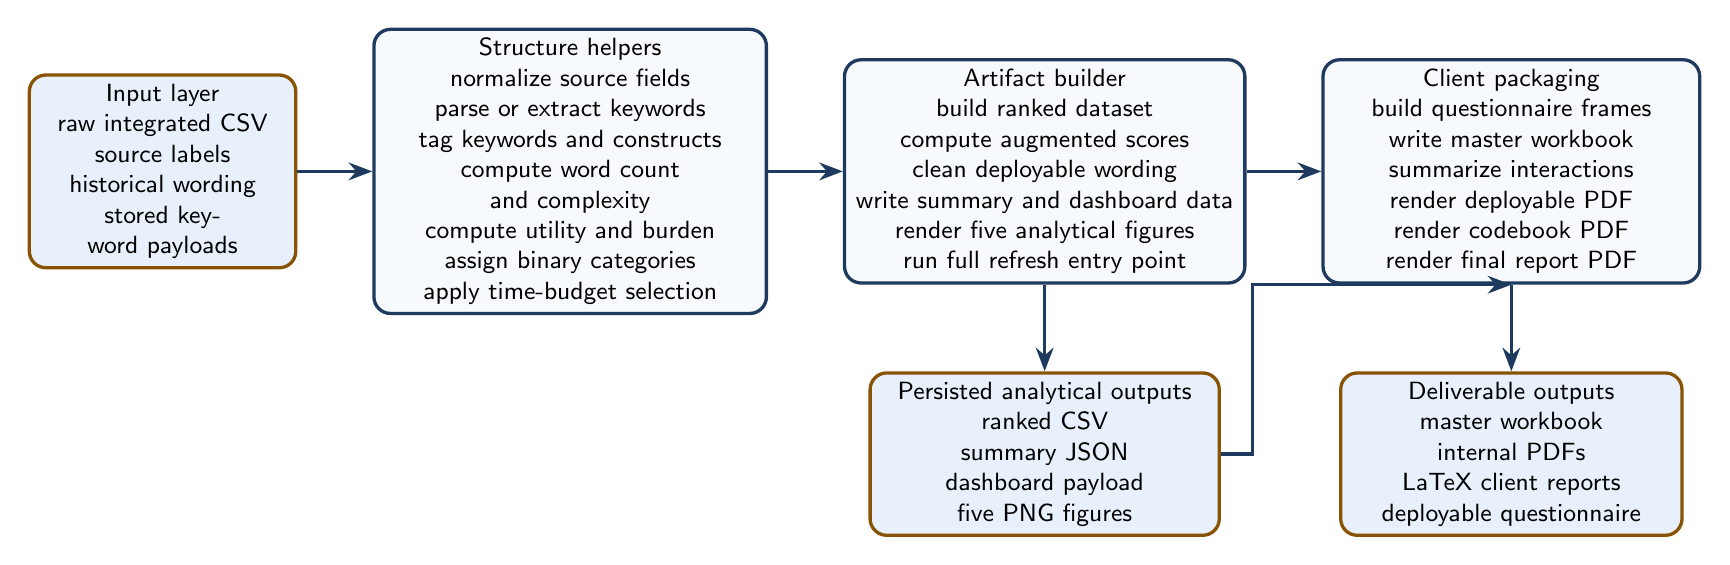
\begin{tikzpicture}[node distance=0.8cm and 0.95cm]
\node[flowresult, text width=3.15cm] (raw) {Input layer\\raw integrated CSV\\source labels\\historical wording\\stored keyword payloads};
\node[flowwide, right=of raw, text width=4.75cm] (structure) {Structure helpers\\normalize source fields\\parse or extract keywords\\tag keywords and constructs\\compute word count and complexity\\compute utility and burden\\assign binary categories\\apply time-budget selection};
\node[flowwide, right=of structure, text width=4.85cm] (artifact) {Artifact builder\\build ranked dataset\\compute augmented scores\\clean deployable wording\\write summary and dashboard data\\render five analytical figures\\run full refresh entry point};
\node[flowwide, right=of artifact, text width=4.55cm] (client) {Client packaging\\build questionnaire frames\\write master workbook\\summarize interactions\\render deployable PDF\\render codebook PDF\\render final report PDF};
\node[flowresult, below=1.1cm of artifact, text width=4.2cm] (artifactout) {Persisted analytical outputs\\ranked CSV\\summary JSON\\dashboard payload\\five PNG figures};
\node[flowresult, below=1.1cm of client, text width=4.1cm] (clientout) {Deliverable outputs\\master workbook\\internal PDFs\\LaTeX client reports\\deployable questionnaire};
\draw[flowarrow] (raw) -- (structure);
\draw[flowarrow] (structure) -- (artifact);
\draw[flowarrow] (artifact) -- (client);
\draw[flowarrow] (artifact) -- (artifactout);
\draw[flowarrow] (artifactout.east) -- ++(0.4,0) |- (client.south);
\draw[flowarrow] (client) -- (clientout);
\end{tikzpicture}
}
\end{document}